\textbf{Single Responsibility Principle}

There are various manifestations of \gls{srp} implemented in the artifacts. One of which is
already mentioned in Figure \ref{fig_modulair_components}, where \gls{srp} is applied to
separate the domain logic from the application, infrastructure and presentation logic. One
could argue that this manifestation is more related to \gls{soc}, considering the high
granularity of the components.

A better example is the separation of handlers that are part of the \gls{ca}
Expander. Each of those handlers executes an isolated part of the expanding process.
Consider the Listing \ref{list_entityexpander} \nameref{list_entityexpander}
\parencite{koks_expandentitieshandlerinteractor_2023} for example. This Handler is solely
responsible for the generation of data entities. 

\begin{figure}[H]
    \centering
    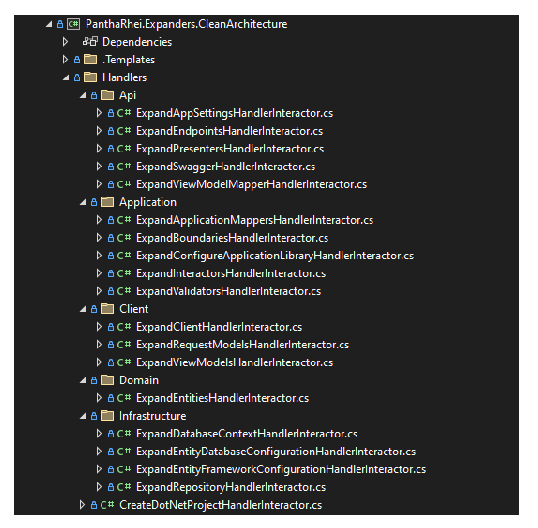
\includegraphics[width=0.6\textwidth]{figures/expander_handlers.pdf}
    \caption[handlers]{Each of the handlers handles an isolated part of the expanding process.}
    \label{fig_handlers}
\end{figure}

\lstinputlisting[
    caption={The \citetitle{koks_expandentitieshandlerinteractor_2023}},
    label={list_entityexpander}]
    {Snippets/ExpandEntitiesHandlerInteractor.cs}